\chapter{Pooling layer}

\subsection*{Structure}

\begin{itemize}
\item Accepts a volume of size

\item Requires two hyperparameters: $W_1 \times H_1 \times D_1$
\begin{itemize}
    \item their spatial extent $F$
    \item the stride $S$
\end{itemize}
\item Produces a volume of size  where: $W_2 \times H_2 \times D_2$
\begin{itemize}
\item $W_2 = \frac{W_1-F}{S}+1$
\item $H_2 = \frac{H_1-F}{S}+1$
\item $D_2 = D_1$
\end{itemize}
\item Introduces zero parameters since it computes a fixed function of the input
\item Note that it is not common to use zero-padding for Pooling layers
\item Has \textbf{NO} parameters
\end{itemize}

\subsection*{Explanation}
It is common to periodically insert a Pooling layer in-between successive Conv layers in a ConvNet architecture. Its function is to progressively reduce the spatial size of the representation to reduce the amount of parameters and computation in the network, and hence to also control overfitting.  This down sampling operations happens on each activation map independently and the volume depth is preserved. The most common way of pooling is max pooling, another one is average pooling but it does not work that well.

The most common form is a pooling layer with filters of size $2 \times 2$ applied with a stride of $2$ downsamples every depth slice in the input by 2 along both width and height, discarding 75\% of the activations. Every MAX operation would in this case be taking a max over $4$ numbers (little $2 \times 2$ region in some depth slice). The depth dimension remains unchanged.

Notice that the pooling layer has NO parameters!!

\begin{figure}[h]
  \centering
  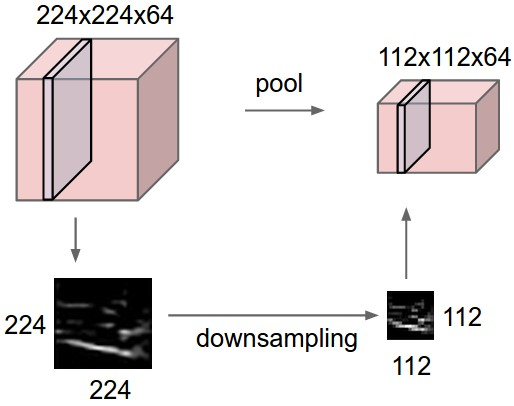
\includegraphics[width=0.4\textwidth]{Images/pool_layer/1.png}
  \caption{ In this example, the input volume of size [$224 \times 224 \times 64$] is pooled with filter size $2$, stride $2$ into output volume of size [$112 \times 112 \times 64$]. Notice that the volume depth is preserved.}
\end{figure}

\begin{figure}[h]
  \centering
  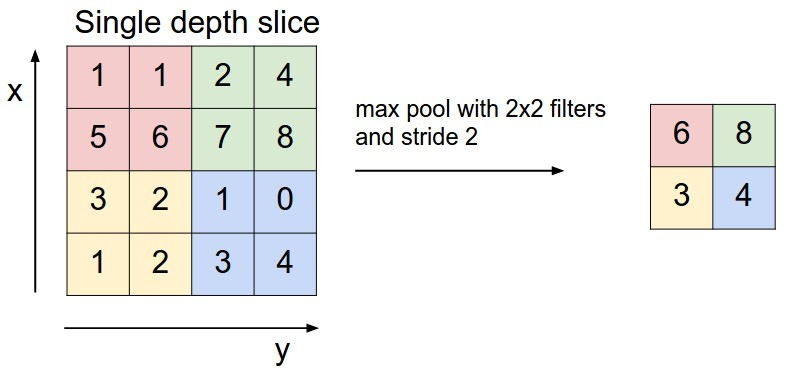
\includegraphics[width=0.45\textwidth]{Images/pool_layer/2.png}
  \caption{The most common downsampling operation is max, giving rise to max pooling, here shown with a stride of $2$. That is, each max is taken over $4$ numbers (little $2 \times 2$ square).}
\end{figure}



\paragraph*{Choosing hyperparameters} There are 2 common setting of the hyperparameters. $F=2, S=2$ that this discards exactly 75\% of the activations in an input volume (due to downsampling by 2 in both width and height). Another slightly less common setting is t. It is very uncommon to see receptive field sizes for max pooling that are larger than 3 because the pooling is then too lossy and aggressive. This usually leads to worse performance.

\paragraph*{Backpropagation} Recall from the backpropagation chapter that the backward pass for a $\text{max}(x, y)$ operation has a simple interpretation as only routing the gradient to the input that had the highest value in the forward pass. Hence, during the forward pass of a pooling layer it is common to keep track of the index of the max activation (sometimes also called the switches) so that gradient routing is efficient during backpropagation.

\paragraph*{Getting rid of pooling} Many people dislike the pooling operation and think that we can get away without it. For example, Striving for Simplicity: The All Convolutional Net proposes to discard the pooling layer in favor of architecture that only consists of repeated CONV layers. To reduce the size of the representation they suggest using larger stride in CONV layer once in a while. Discarding pooling layers has also been found to be important in training good generative models, such as variational autoencoders (VAEs) or generative adversarial networks (GANs). It seems likely that future architectures will feature very few to no pooling layers.